\documentclass[]{IEEEtran}
% some very useful LaTeX packages include:
%\usepackage{cite}      
\usepackage{graphicx}   
\usepackage{subfigure} 
\usepackage{url}       
\usepackage{amsmath}    
\usepackage{caption2}
% Your document starts here!
\begin{document}

% Define document title and author
	\title{Weekly Report}
	\author{Adviser: Prof. Yang Wen \\Student: Cheng Wensheng\\ Period: 2018.6.4-6.10
	}
	\markboth{Visual Information Processing Group}{}
	\maketitle

% Write abstract here
\begin{abstract}
	This week I mainly put my effort on treating Prof. Marcello, and taking the machine learning course.
\end{abstract}

% Each section begins with a \section{title} command
\section{Machine Learning Course}
	% \PARstart{}{} creates a tall first letter for this first paragraph
	\PARstart{T}{his} week we invited Prof. Marcello to give a class of machine learning and big data.
	\begin{itemize}
		\item Prof. Marcello is a professor of Computer Science at the University of Venice, Italy. He serves on the editorial boards of IEEE TPAMI. He has initiated several conferences series as Program Chair (EMMCVPR, IWCV, SIMBAD) and served as a General Chair for ICCV 2017 and will serve as a Area Chair for ECCV 2018. He is slao an IEEE Fellow and IAPR Fellow.
		\item This class includes basic concepts of machine learning, such as SVM, VC dimension, clustering. Since he is familiar with graph models and game theory, these parts are more intriguing.
		\item When introduce classes, foreign professors prefer to give us a historical view of these concepts. In this way, students can understand these notions better and can grasp these ideas in an intuitive way.
		\item About communication, since he is not a native speaker, so the speed is not fast. There is no problem of talking with him. Still, I need to enlarge my vocabulary to be more fluent.
	\end{itemize}

	There are some slides that impressed me a lot. Fig.~\ref{fig:mp} is the bias question. Fig.~\ref{fig:ss} is the adversarial sample.

\newpage
\begin{figure}[!hbt]
%		 Center the figure.
		\vspace{0.1cm}
%		\hspace{50cm}
%		\begin{center}
			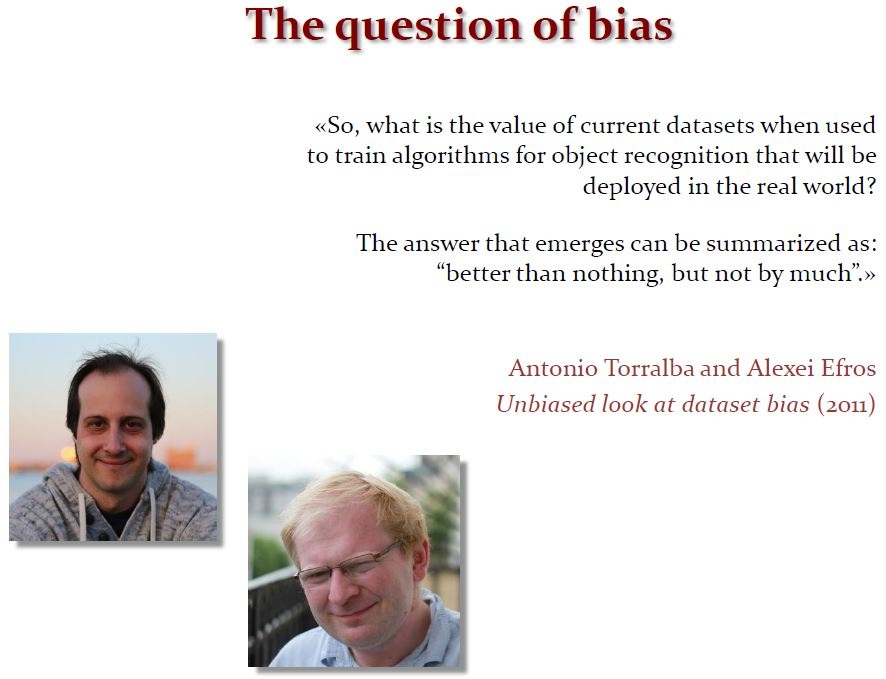
\includegraphics[width=0.7\columnwidth]{bias}
				%		 Create a subtitle for the figure.
			\caption{Bias question}
			\label{fig:mp}
			\vspace{0.3cm}
		    \hspace{0.5cm}
			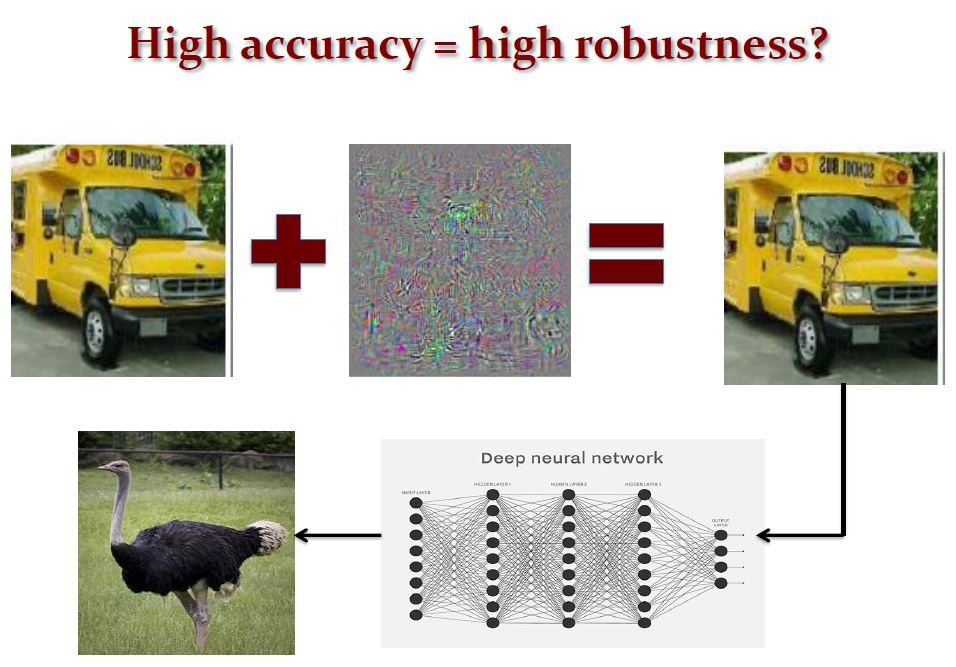
\includegraphics[width=0.7\columnwidth]{ad}
				%Create a subtitle for the figure.
			\caption{Adversarial sample}
			\label{fig:ss}
%		\end{center}
	\end{figure}

% Now we need a bibliography:
%\begin{thebibliography}{5}
%
%	%Each item starts with a \bibitem{reference} command and the details thereafter.
%	\bibitem{HOP96} % Transaction paper
%	J.~Hagenauer, E.~Offer, and L.~Papke. Iterative decoding of binary block
%	and convolutional codes. {\em IEEE Trans. Inform. Theory},
%	vol.~42, no.~2, pp.~429–-445, Mar. 1996.
%
%	\bibitem{MJH06} % Conference paper
%	T.~Mayer, H.~Jenkac, and J.~Hagenauer. Turbo base-station cooperation for intercell interference cancellation. {\em IEEE Int. Conf. Commun. (ICC)}, Istanbul, Turkey, pp.~356--361, June 2006.
%
%	\bibitem{Proakis} % Book
%	J.~G.~Proakis. {\em Digital Communications}. McGraw-Hill Book Co.,
%	New York, USA, 3rd edition, 1995.
%
%	\bibitem{talk} % Web document
%	F.~R.~Kschischang. Giving a talk: Guidelines for the Preparation and Presentation of Technical Seminars.
%	\url{http://www.comm.toronto.edu/frank/guide/guide.pdf}.
%
%	\bibitem{5}
%	IEEE Transactions \LaTeX and Microsoft Word Style Files.
%	\url{http://www.ieee.org/web/publications/authors/transjnl/index.html}
%
%\end{thebibliography}

% Your document ends here!
\end{document}